\documentclass[a4paper]{article}
\usepackage{graphicx} %Required for diagrams
\usepackage[bookmarks=true]{hyperref}
\usepackage{bookmark}%Required to do pdf bookmarking
\usepackage[margin=1.2in]{geometry}
\usepackage{float}
\usepackage{caption}
\usepackage{hyperref}%Required for referencing website pages
\usepackage[english]{babel}
%\usepackage[utf8x]{inputenc}
\usepackage{graphicx}
\usepackage{dcolumn}
\usepackage[table]{xcolor}
%\usepackage[colorinlistoftodos]{todonotes}

\title{Plan for Software Aspects of Certification}
\author{Baobab Team}

\begin{document}
\newpage

\input{./TitlePage.tex}
\newpage

\section{Product Backlog}

\begin{figure}[H]
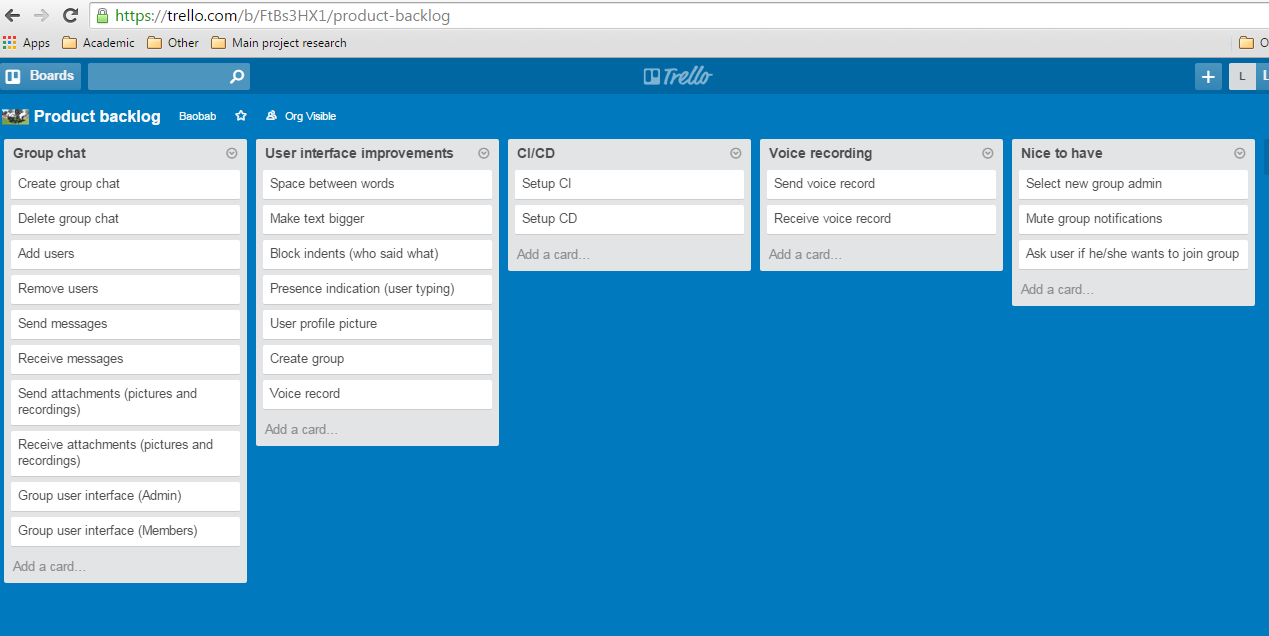
\includegraphics[width=1\linewidth]{./pictures/backlog.jpg}\\
\caption{\label{fig:Product Backlog}Product Backlog}
\end{figure}

\href{https://trello.com/b/FtBs3HX1}{Click-able link to Product Backlog on Trello}
\newpage

\section{Sprint Backlog}

\begin{figure}[H]
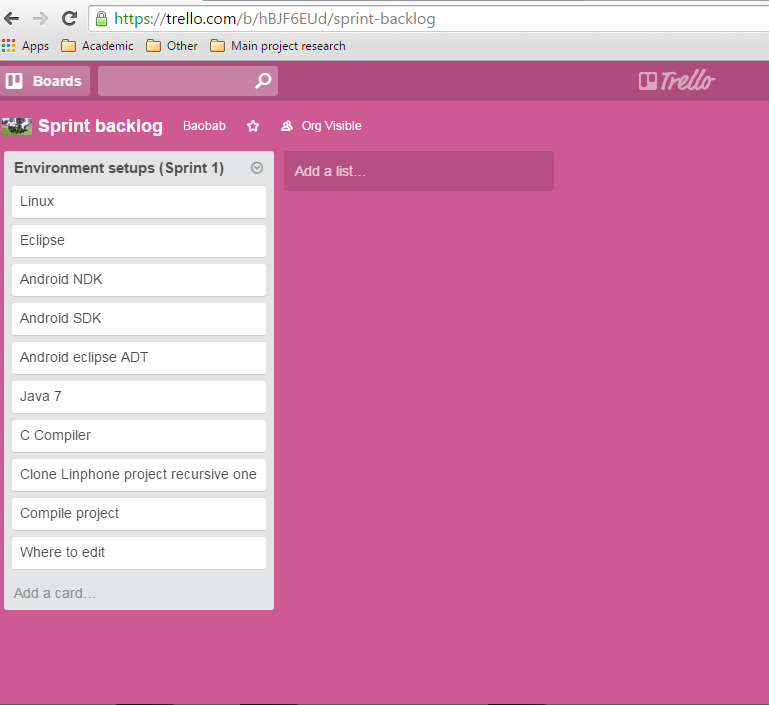
\includegraphics[width=1\linewidth]{./pictures/sprintbacklog.jpg}\\
\caption{\label{fig:Sprint Backlog}Sprint Backlog}
\end{figure}

\href{https://trello.com/b/hBJF6EUd}{Click-able link to Sprint Backlog on Trello}
\newpage

\section{Sprint Review}

\subsection{Participants}
\begin{table}[h]
\centering
\caption{Scrum User Roles}
\label{User Roles}
\begin{center} \rowcolors{1}{green}{pink}
\begin{tabular}{| l | c | r |}
\hline
Scrum master  & Potego Mello\\ \hline
Client representative  & Patience Mtsweni\\ \hline
UX developer  & Lutfiyya Razak\\ \hline
Backend developer  & Ephiphania Munava\\\hline
Crypto developer  & Tsepo Ntsaba and Lerato Molokomme\\ \hline
CI / CD support  & Patience Mtsweni \\ 
\hline
\end{tabular}
\end{center}
\end{table}

\subsection{Sprint Summary}
\begin{table}[h]
\centering
\caption{Sprint Summary}
\begin{tabular}{| l | c | c | r |}
\hline
Sprint Number & Sprint & Start Date & End Date\\ \hline
1 & Environment Setup & 23 June 2015 & 30 June 2015 \\
\hline
\end{tabular}
\end{table}


\subsection{Software Architecture}
\textbf{Description: }We did not modify the software architecture. \\

\subsection{SprintSummary}
Environment Setup 
\subsubsection{What we got done: }
\textbf{Description: }We pulled the environment setup sprint and discussed what we are going to accomplish in this sprint. \\

\begin{table}[h]
\centering
\caption{Completed Work}
\begin{tabular}{| l | c | c | c | r |}
\hline 
Date Complete & Implemented in production quality & Tested & Integrated & Documented\\ \hline
23 June 2015 & Yes & Product Backlog & Not Applicable & \href{https://trello.com/b/FtBs3HX1}{Click-able link to Product Backlog on Trello}\\ \hline
23 June 2015 & Yes & Environment Setup Sprint & Not Applicable & \href{https://trello.com/b/hBJF6EUd}{Click-able link to Sprint Backlog on Trello}\\ 
\hline
\end{tabular}
\end{table}

\subsection{What we plan to do next:}
\textbf{Description: }We will pull the CI/CD Setup from Product Backlog. \\

\begin{table}[h]
\centering
\caption{Work to complete}
\begin{tabular}{| l | c | c | r |}
\hline
Date to begin  & Task to implement & Date to complete\\ \hline
24 June 2015 & CI/CD Setup & 5 July 2015 \\
\hline
\end{tabular}
\end{table}

\end{document}